Nesta seção, são apresentados e discutidos os principais resultados obtidos com a aplicação do sistema fuzzy Takagi-Sugeno para aproximação da função alvo proposta. São analisados o comportamento das funções de pertinência, a qualidade das aproximações para diferentes configurações do modelo (ordem zero e primeira ordem), o impacto da otimização dos consequentes e a comparação dos desempenhos por meio do RMSE. As figuras e tabelas a seguir ilustram e fundamentam a análise dos resultados.

\subsection{Geração do Conjunto de Dados}

Para a aproximação da função alvo, foram gerados $200$ pontos uniformemente espaçados no intervalo $x \in [0, 10]$. Para cada valor de $x$, foi calculado o valor correspondente da função não linear:
\[
f(x) = e^{-x/5} \cdot \sin(3x) + 0.5 \cdot \sin(x)
\]
A geração dos dados e a plotagem do gráfico foram realizadas em Python, utilizando as bibliotecas NumPy e Matplotlib.

A Figura~\ref{fig:fx} apresenta o gráfico da função alvo no intervalo considerado, evidenciando seu comportamento não linear e oscilatório.

\begin{figure}[!ht]
    \centering
    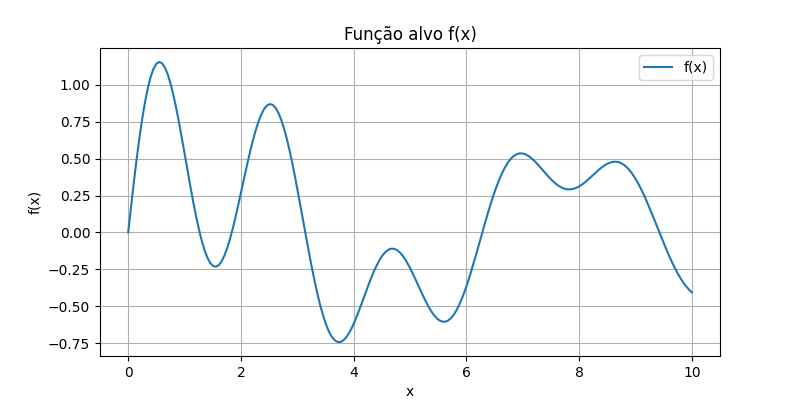
\includegraphics[width=0.45\textwidth]{../img/fx_takagi_sugeno2.png}
    \caption{Função alvo $f(x)$ no intervalo $[0, 10]$.}
    \label{fig:fx}
\end{figure}

\subsection{Estrutura do Sistema Fuzzy Takagi-Sugeno}

O sistema fuzzy Takagi-Sugeno desenvolvido neste trabalho possui a seguinte estrutura:

\begin{itemize}
    \item \textbf{Variável de entrada:} $x \in [0, 10]$
    \item \textbf{Saída:} $y \approx f(x)$
    \item \textbf{Regras:} 3 regras principais (Baixo, Médio, Alto)
    \item \textbf{Funções de pertinência:} gaussianas, triangulares e trapezoidais
    \item \textbf{Consequentes:} constantes (ordem zero) ou lineares (primeira ordem)
    \item \textbf{Operador de agregação:} soma ponderada pelas pertinências
\end{itemize}

\subsection{Funções de Pertinência}

Para a modelagem fuzzy, foram utilizadas três famílias de funções de pertinência: gaussianas, triangulares e trapezoidais. O objetivo é comparar o desempenho do sistema em relação ao tipo de função de pertinência adotada. Foram definidos $n=20$ conjuntos fuzzy ao longo do intervalo $x \in [0, 10]$, com parâmetros calculados para garantir cobertura uniforme do domínio.

As funções de pertinência são matematicamente definidas por:

\begin{itemize}
    \item \textbf{Gaussiana:} $\mu(x) = \exp\left(-\frac{1}{2}\left(\frac{x-c}{\sigma}\right)^2\right)$
    \item \textbf{Triangular:} $\mu(x) = \max\left(0, \min\left(\frac{x-a}{b-a}, \frac{c-x}{c-b}\right)\right)$
    \item \textbf{Trapezoidal:} $\mu(x) = \max\left(0, \min\left(\frac{x-a}{b-a}, 1, \frac{d-x}{d-c}\right)\right)$
\end{itemize}

A Figura~\ref{fig:fx} mostra a função alvo $f(x)$, enquanto as Figuras~\ref{fig:mf_gaussiana}, \ref{fig:mf_triangular} e \ref{fig:mf_trapezoidal} apresentam, respectivamente, as funções de pertinência gaussianas, triangulares e trapezoidais utilizadas no sistema fuzzy.

\begin{figure}[!ht]
    \centering
    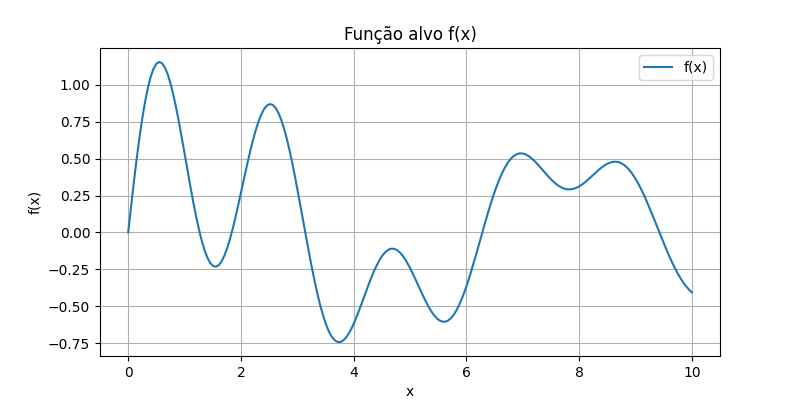
\includegraphics[width=0.48\textwidth]{../img/fx_takagi_sugeno2.png}
    \caption{Função alvo $f(x)$ no intervalo $[0, 10]$.}
    \label{fig:fx}
\end{figure}

\begin{figure}[!ht]
    \centering
    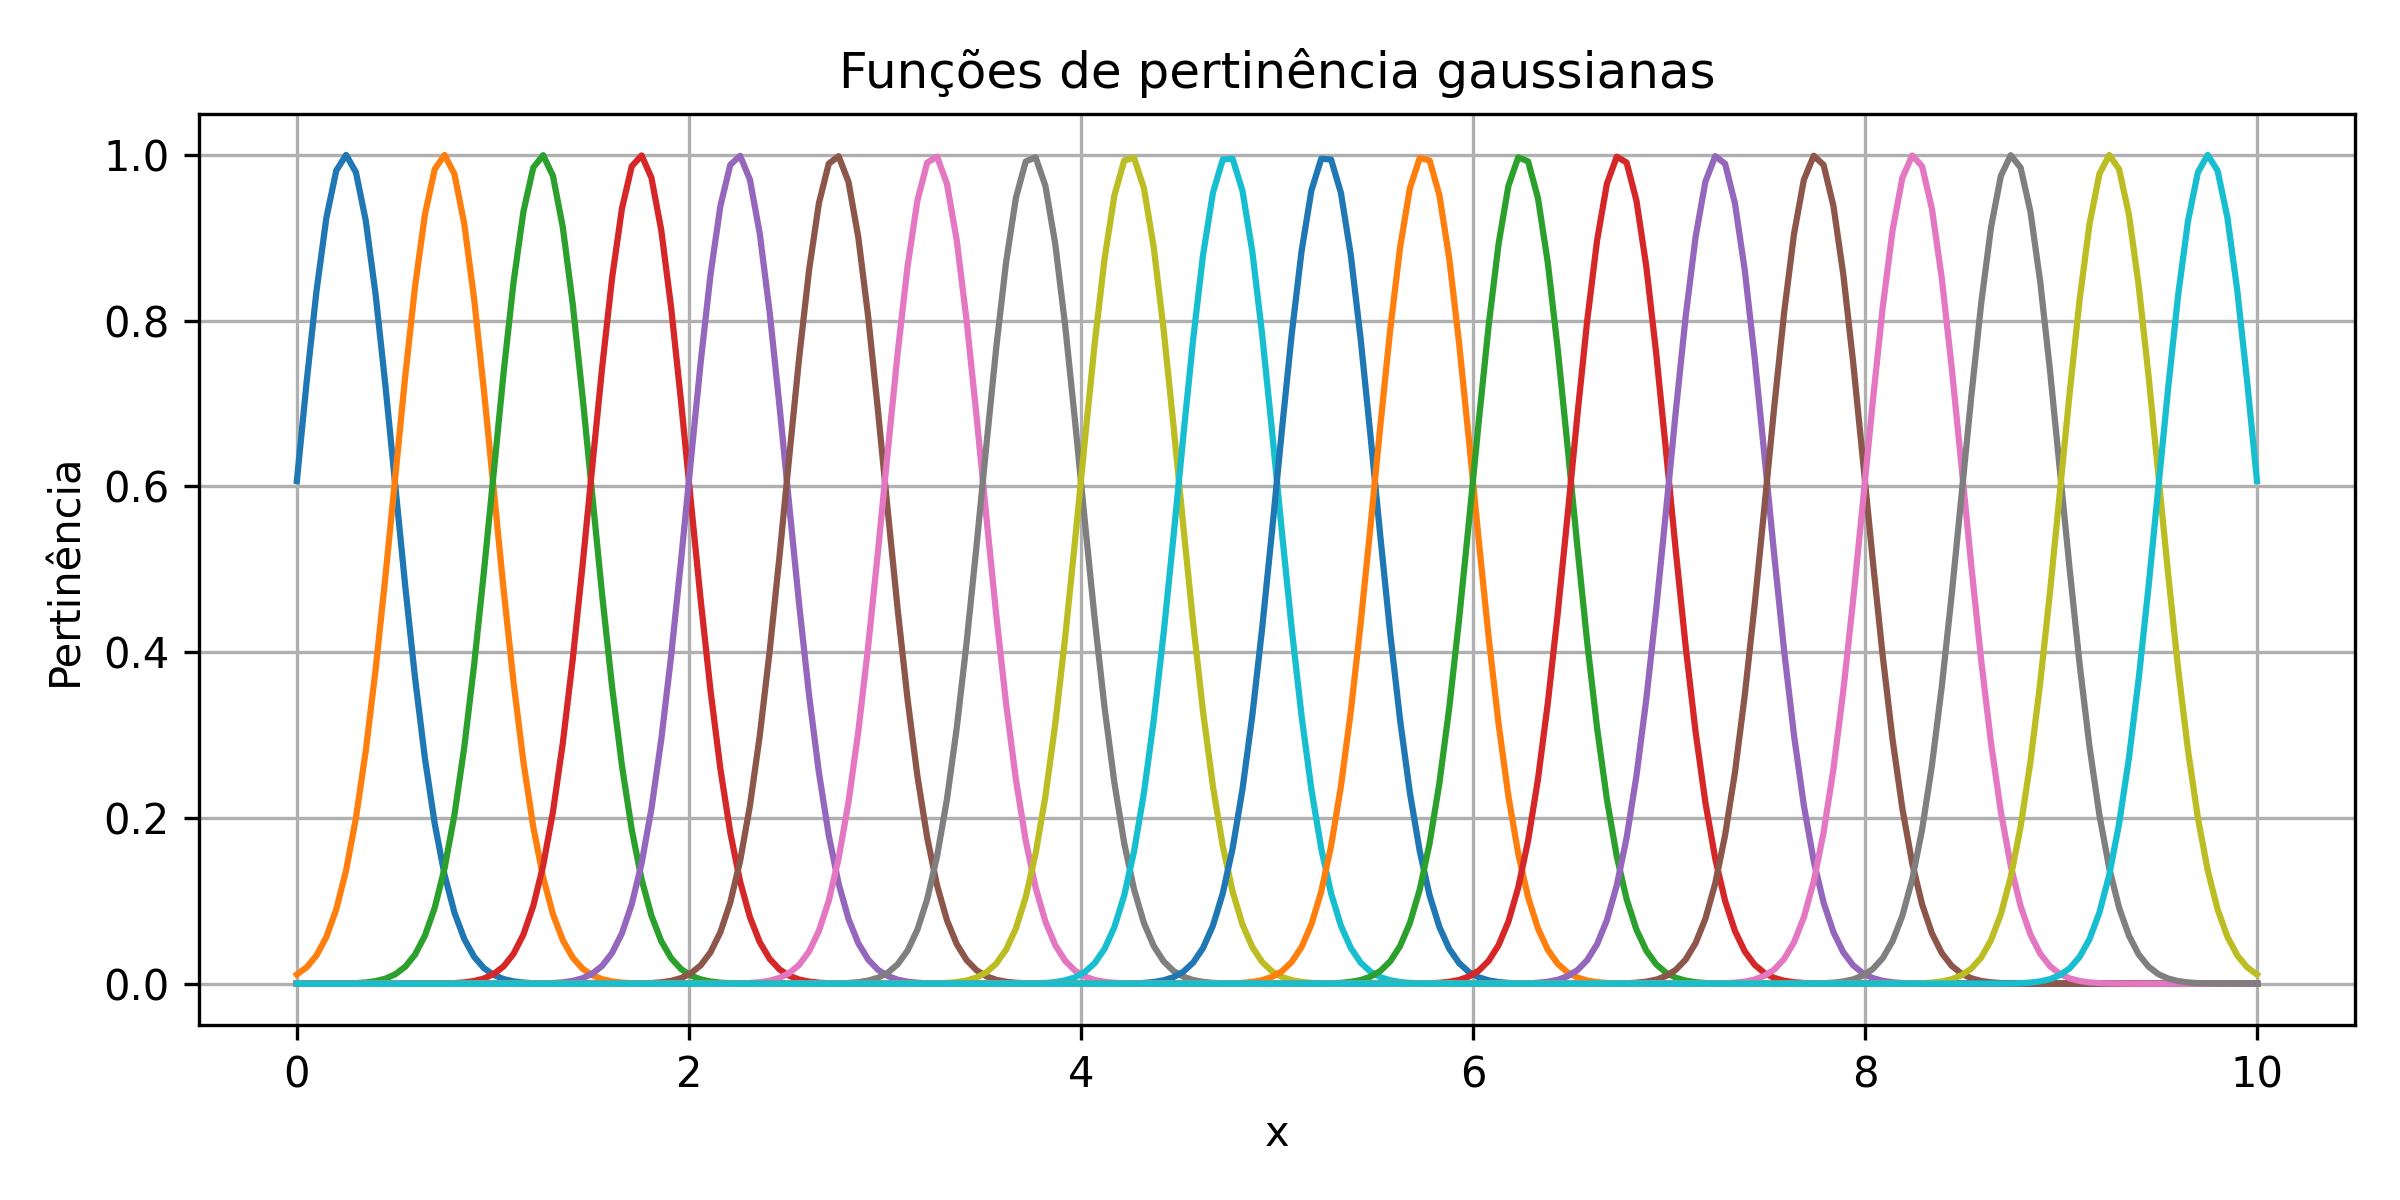
\includegraphics[width=0.48\textwidth]{../img/funcoes_de_pertinencia_gaussianas.png}
    \caption{Funções de pertinência gaussianas utilizadas no sistema fuzzy.}
    \label{fig:mf_gaussiana}
\end{figure}

\begin{figure}[!ht]
    \centering
    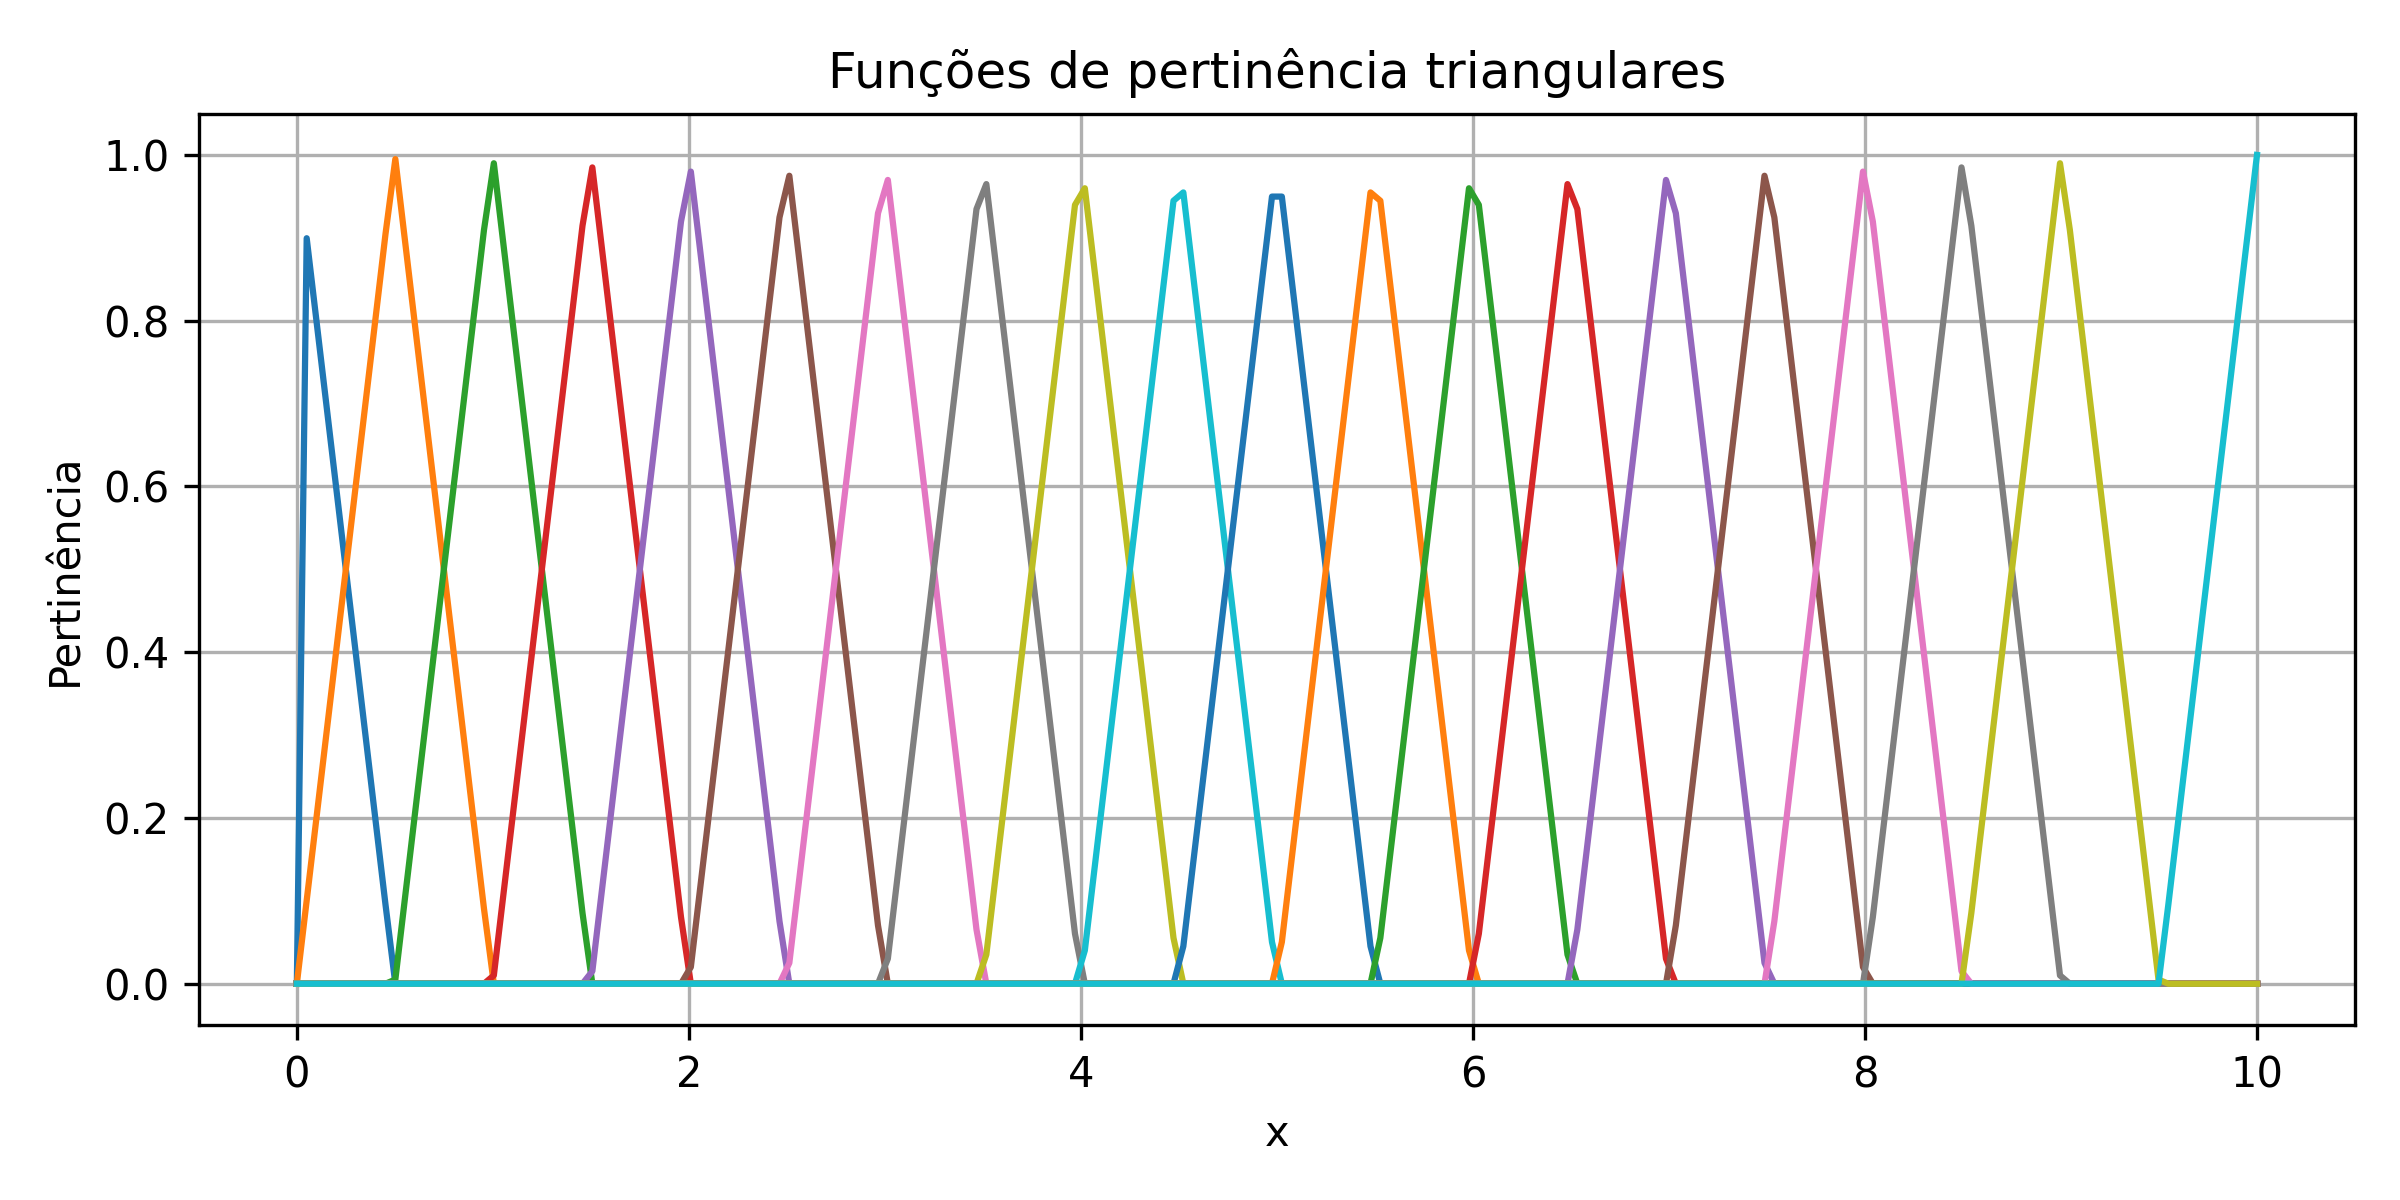
\includegraphics[width=0.48\textwidth]{../img/funcoes_de_pertinencia_triangulares.png}
    \caption{Funções de pertinência triangulares utilizadas no sistema fuzzy.}
    \label{fig:mf_triangular}
\end{figure}

\begin{figure}[!ht]
    \centering
    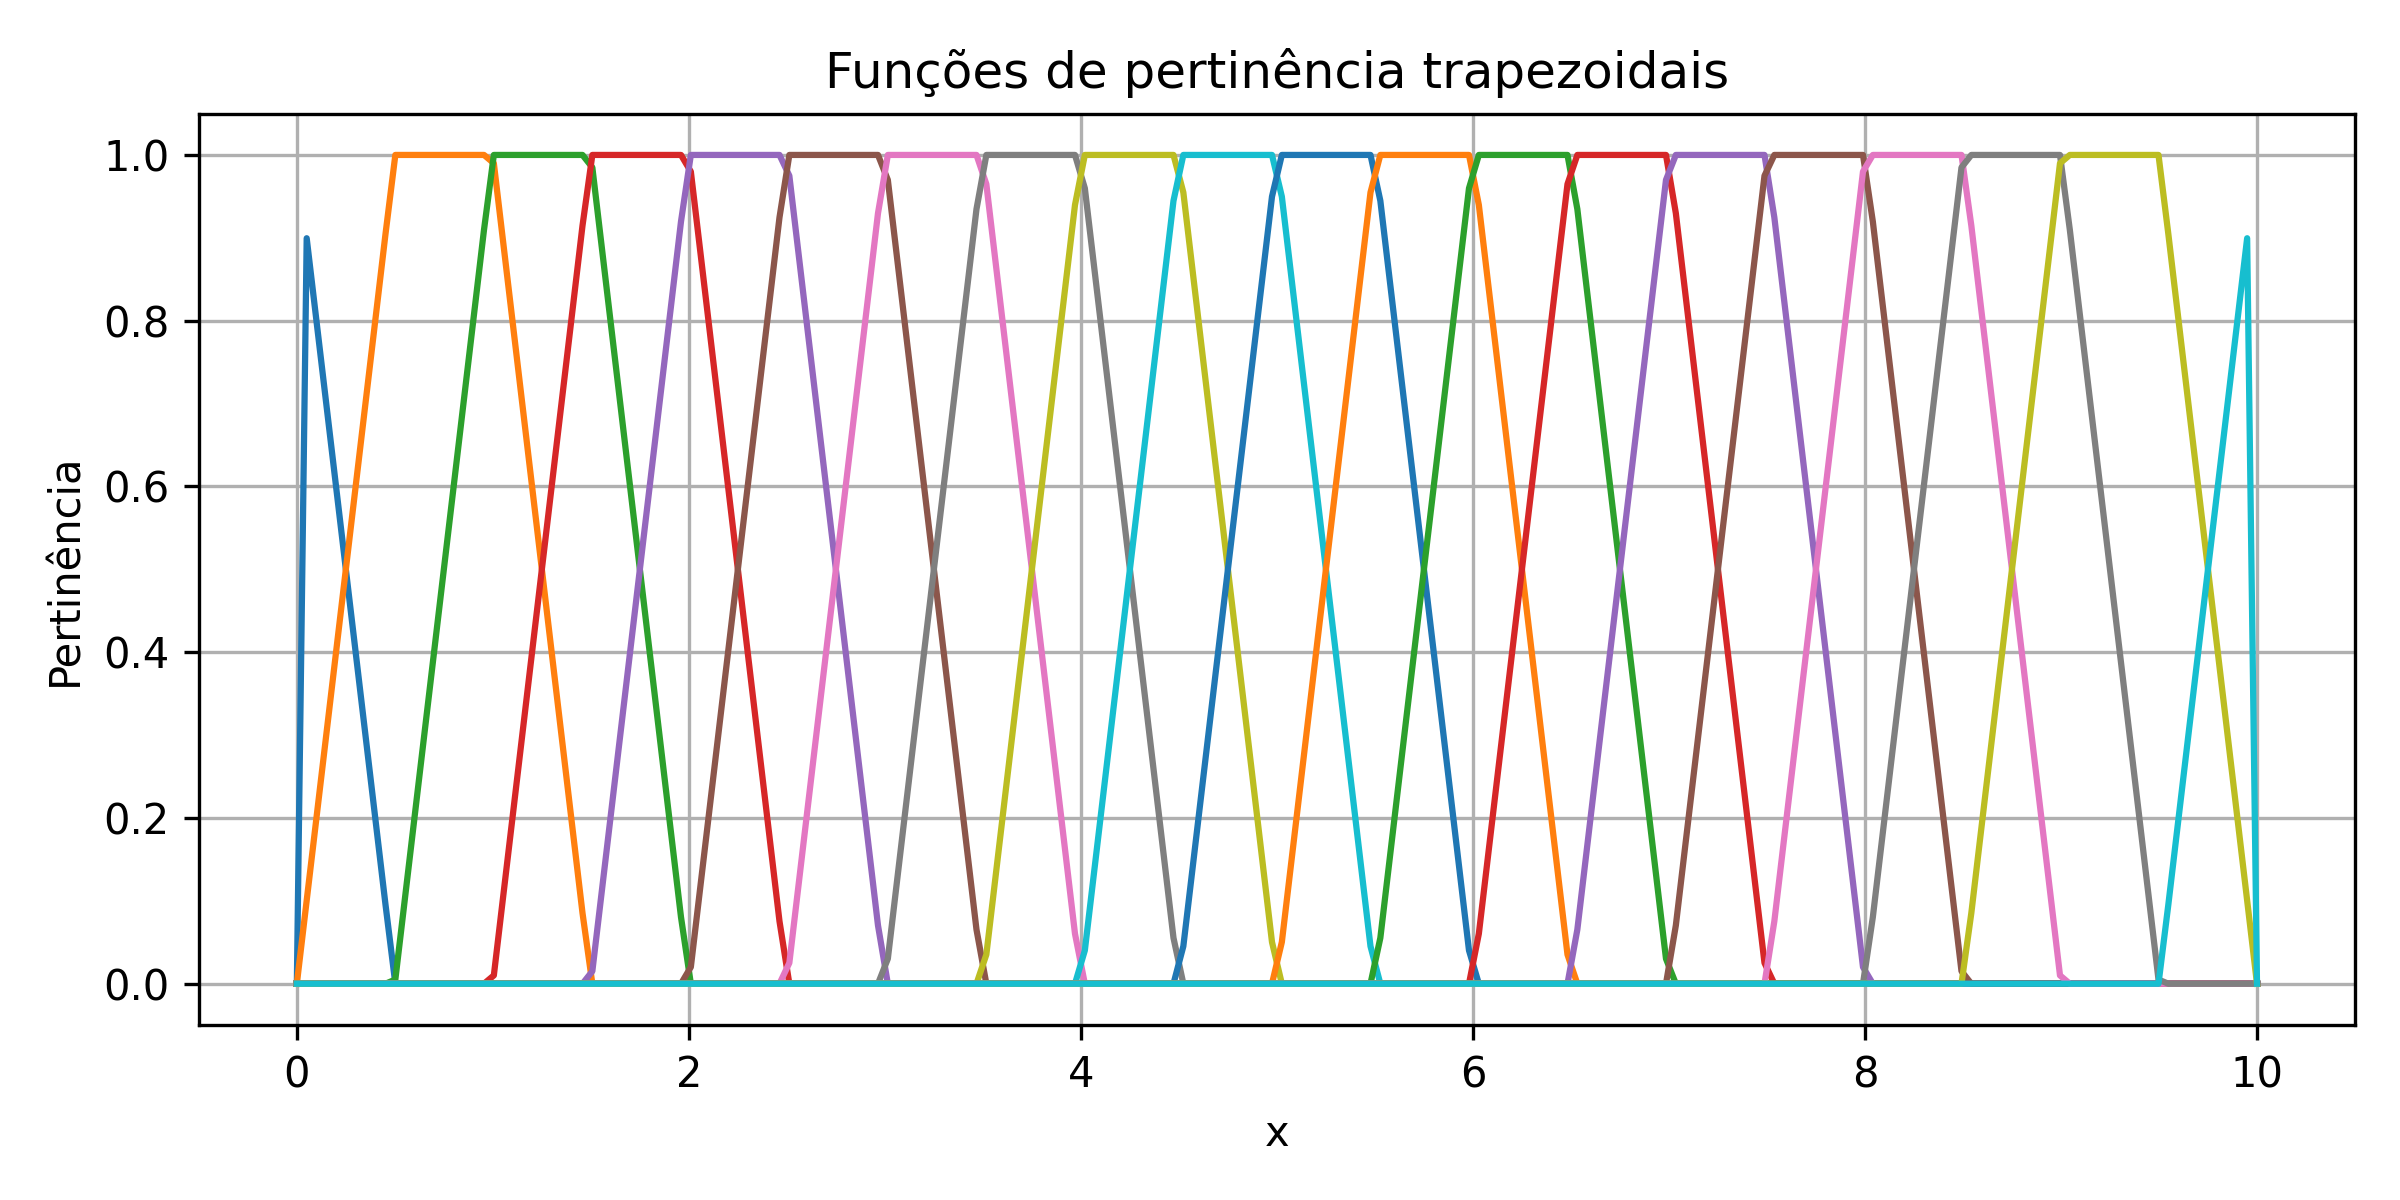
\includegraphics[width=0.48\textwidth]{../img/funcoes_de_pertinencia_trapezoidais.png}
    \caption{Funções de pertinência trapezoidais utilizadas no sistema fuzzy.}
    \label{fig:mf_trapezoidal}
\end{figure}

As figuras foram geradas a partir do código Python, utilizando as bibliotecas NumPy e Matplotlib. Cada tipo de função de pertinência foi visualizado separadamente para facilitar a análise e comparação.

\subsection{Takagi-Sugeno de Ordem Zero}

No sistema Takagi-Sugeno de ordem zero, cada regra fuzzy possui um consequente constante. A saída do sistema é calculada como a média ponderada dos consequentes, utilizando os graus de pertinência como pesos. A expressão matemática para a saída $y(x)$ é:

\[
y(x) = \frac{\sum_{i=1}^{n} \mu_i(x) \cdot c_i}{\sum_{i=1}^{n} \mu_i(x)}
\]

onde:
\begin{itemize}
    \item $\mu_i(x)$: grau de pertinência do $i$-ésimo conjunto fuzzy para a entrada $x$;
    \item $c_i$: consequente constante associado à $i$-ésima regra;
    \item $n$: número total de regras.
\end{itemize}

Os consequentes $c_i$ são calculados de modo a minimizar o erro em relação à função alvo, conforme:

\[
c_i = \frac{\sum_{k=1}^{N} \mu_i(x_k) \cdot f(x_k)}{\sum_{k=1}^{N} \mu_i(x_k)}
\]

onde $x_k$ são os pontos do conjunto de dados e $f(x_k)$ os valores da função alvo.

A Figura~\ref{fig:ts_ordem_zero_todas} apresenta a aproximação da função alvo utilizando o sistema Takagi-Sugeno de ordem zero para diferentes tipos de funções de pertinência.

\begin{figure}[!ht]
    \centering
    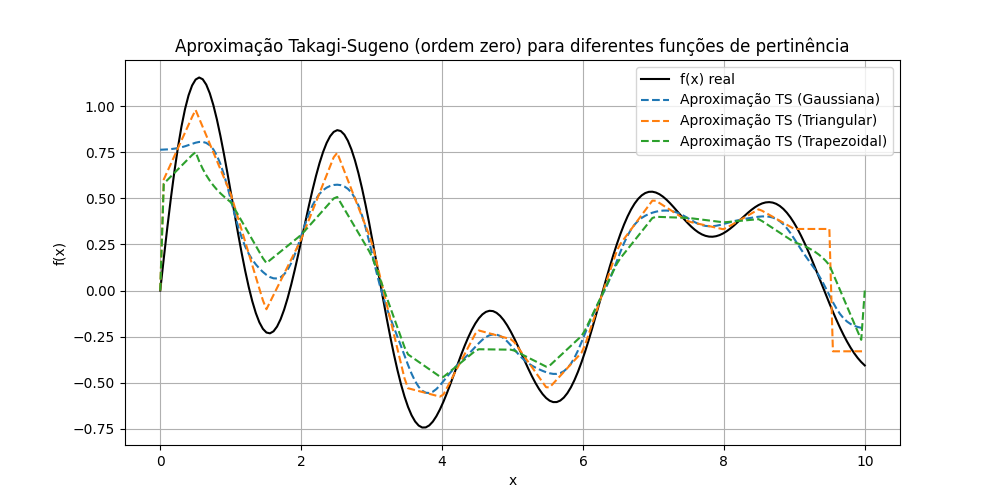
\includegraphics[width=0.45\textwidth]{../img/fx_aprox_ordem_zero_todas_takagi_sugeno2.png}
    \caption{Aproximação Takagi-Sugeno (ordem zero) para diferentes funções de pertinência.}
    \label{fig:ts_ordem_zero_todas}
\end{figure}

As Figuras~\ref{fig:ts_ordem_zero_gaussiana}, \ref{fig:ts_ordem_zero_triangular} e \ref{fig:ts_ordem_zero_trapezoidal} mostram detalhadamente a aproximação para cada tipo de função de pertinência:

\begin{figure}[!ht]
    \centering
    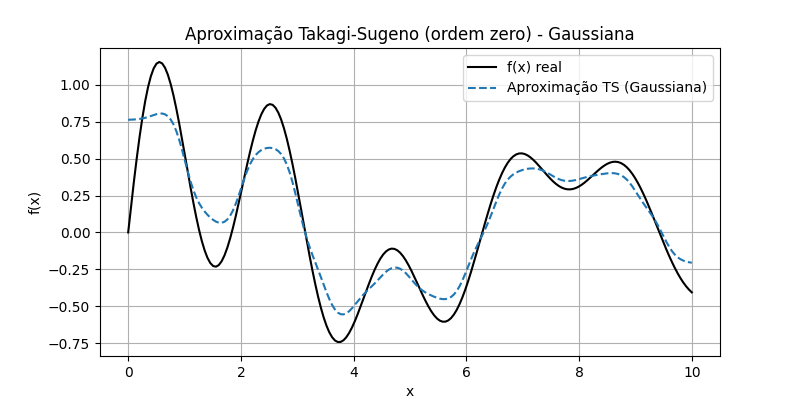
\includegraphics[width=0.45\textwidth]{../img/fx_aprox_ordem_zero_gaussiana_takagi_sugeno2.png}
    \caption{Aproximação Takagi-Sugeno (ordem zero) - Gaussiana.}
    \label{fig:ts_ordem_zero_gaussiana}
\end{figure}

\begin{figure}[!ht]
    \centering
    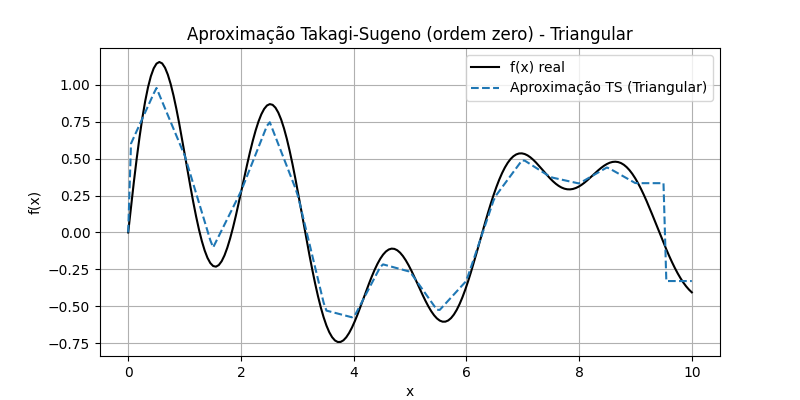
\includegraphics[width=0.45\textwidth]{../img/fx_aprox_ordem_zero_triangular_takagi_sugeno2.png}
    \caption{Aproximação Takagi-Sugeno (ordem zero) - Triangular.}
    \label{fig:ts_ordem_zero_triangular}
\end{figure}

\begin{figure}[!ht]
    \centering
    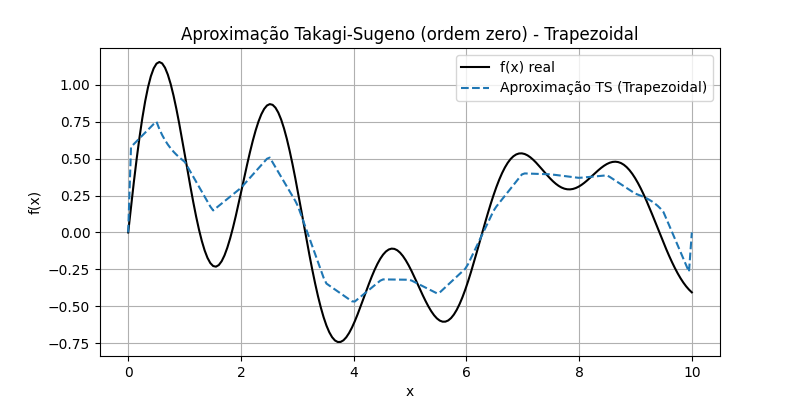
\includegraphics[width=0.45\textwidth]{../img/fx_aprox_ordem_zero_trapezoidal_takagi_sugeno2.png}
    \caption{Aproximação Takagi-Sugeno (ordem zero) - Trapezoidal.}
    \label{fig:ts_ordem_zero_trapezoidal}
\end{figure}


\subsection{Takagi-Sugeno de Primeira Ordem}

No sistema Takagi-Sugeno de primeira ordem, cada regra fuzzy possui um consequente linear, ou seja, a saída de cada regra é dada por uma função do tipo $y = a_i x + b_i$. Os parâmetros $a_i$ e $b_i$ de cada regra são ajustados por mínimos quadrados ponderados, considerando os graus de pertinência como pesos.

A saída global do sistema é calculada como a média ponderada das saídas das regras:

\[
y(x) = \frac{\sum_{i=1}^{n} \mu_i(x) \cdot (a_i x + b_i)}{\sum_{i=1}^{n} \mu_i(x)}
\]

onde:
\begin{itemize}
    \item $\mu_i(x)$: grau de pertinência do $i$-ésimo conjunto fuzzy para a entrada $x$;
    \item $a_i$, $b_i$: coeficientes do consequente linear da $i$-ésima regra;
    \item $n$: número total de regras.
\end{itemize}

Os parâmetros $a_i$ e $b_i$ são encontrados resolvendo o sistema de mínimos quadrados ponderados para cada função de pertinência, conforme:

\[
\begin{bmatrix}
a_i \\
b_i
\end{bmatrix}
= \left( X^T W_i X \right)^{-1} X^T W_i y
\]

em que $X$ é a matriz de entrada (com coluna de $x$ e coluna de 1's), $W_i$ é a matriz diagonal dos pesos (graus de pertinência) e $y$ é o vetor de valores da função alvo.

A Figura~\ref{fig:ts_1ordem_todas} apresenta a aproximação da função alvo utilizando o sistema Takagi-Sugeno de primeira ordem para diferentes tipos de funções de pertinência.

\begin{figure}[!ht]
    \centering
    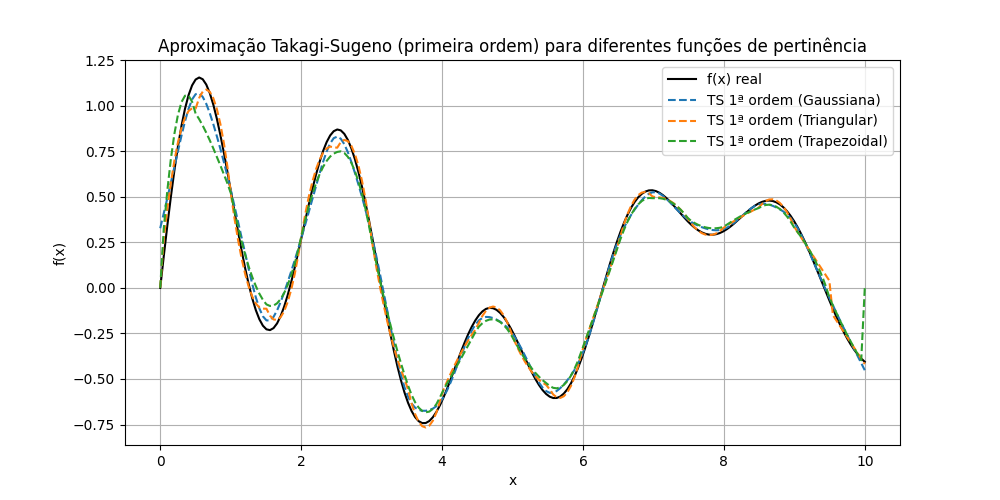
\includegraphics[width=0.45\textwidth]{../img/fx_aprox_1ordem_todas_takagi_sugeno2.png}
    \caption{Aproximação Takagi-Sugeno (primeira ordem) para diferentes funções de pertinência.}
    \label{fig:ts_1ordem_todas}
\end{figure}

As Figuras~\ref{fig:ts_1ordem_gaussiana}, \ref{fig:ts_1ordem_triangular} e \ref{fig:ts_1ordem_trapezoidal} mostram detalhadamente a aproximação para cada tipo de função de pertinência:

\begin{figure}[!ht]
    \centering
    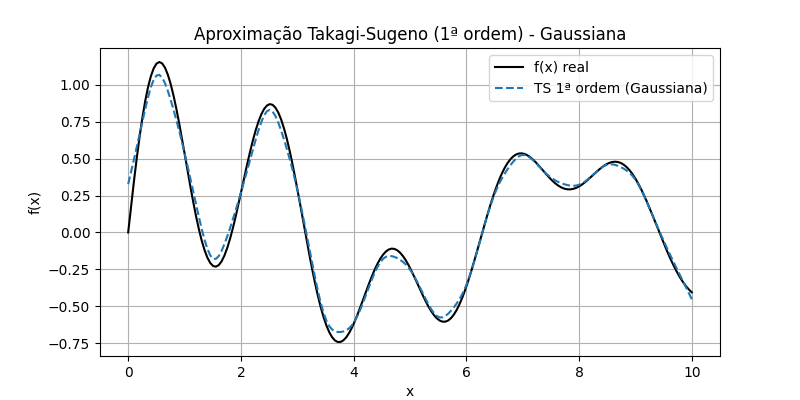
\includegraphics[width=0.45\textwidth]{../img/fx_aprox_1ordem_gaussiana_takagi_sugeno2.png}
    \caption{Aproximação Takagi-Sugeno (primeira ordem) - Gaussiana.}
    \label{fig:ts_1ordem_gaussiana}
\end{figure}

\begin{figure}[!ht]
    \centering
    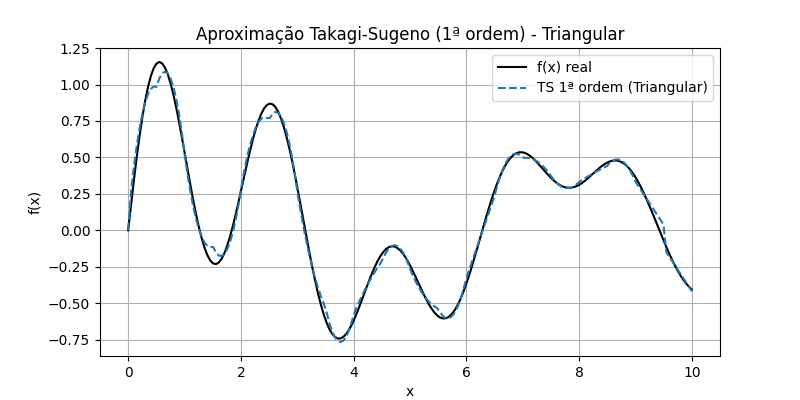
\includegraphics[width=0.45\textwidth]{../img/fx_aprox_1ordem_triangular_takagi_sugeno2.png}
    \caption{Aproximação Takagi-Sugeno (primeira ordem) - Triangular.}
    \label{fig:ts_1ordem_triangular}
\end{figure}

\begin{figure}[!ht]
    \centering
    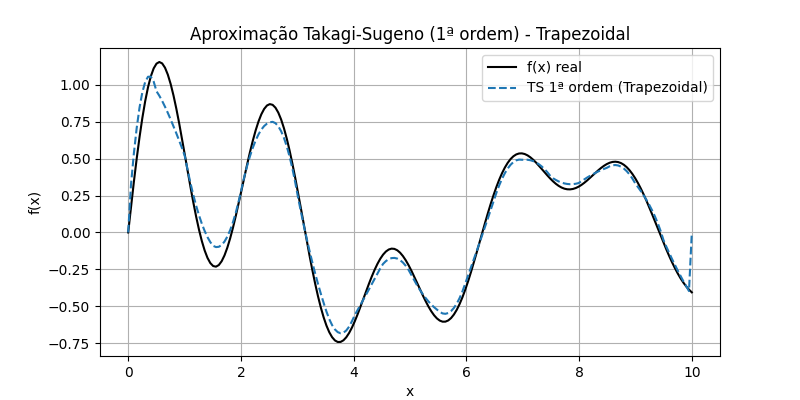
\includegraphics[width=0.45\textwidth]{../img/fx_aprox_1ordem_trapezoidal_takagi_sugeno2.png}
    \caption{Aproximação Takagi-Sugeno (primeira ordem) - Trapezoidal.}
    \label{fig:ts_1ordem_trapezoidal}
\end{figure}

Observa-se que, ao utilizar consequentes lineares, o sistema fuzzy é capaz de obter uma aproximação ainda mais precisa da função alvo, especialmente quando comparado ao modelo de ordem zero.
Observa-se que, ao utilizar consequentes lineares, o sistema fuzzy é capaz de obter uma aproximação ainda mais precisa da função alvo, especialmente quando comparado ao modelo de ordem zero.

\subsection{Avaliação de Desempenho}

Para avaliar o desempenho dos modelos Takagi-Sugeno de ordem zero e de primeira ordem, foi utilizado o erro quadrático médio (RMSE) entre a saída do sistema fuzzy e a função alvo $f(x)$. O RMSE é calculado por:

\[
\mathrm{RMSE} = \sqrt{\frac{1}{N} \sum_{k=1}^{N} \left( y_k - \hat{y}_k \right)^2}
\]

onde $y_k$ representa o valor real da função alvo e $\hat{y}_k$ o valor estimado pelo modelo.

Os resultados obtidos para cada configuração de função de pertinência estão apresentados na Tabela~\ref{tab:rmse_ts}.

\begin{table}[H]
    \centering
    \caption{RMSE para os modelos Takagi-Sugeno de ordem zero e primeira ordem.}
    \label{tab:rmse_ts}
    \begin{tabular}{lcc}
        \toprule
        \textbf{Função de Pertinência} & \textbf{Ordem Zero} & \textbf{Primeira Ordem} \\
        \midrule
        Gaussiana   & 0.16166 & 0.05076 \\
        Triangular  & 0.12616 & 0.03851 \\
        Trapezoidal & 0.21384 & 0.08118 \\
        \bottomrule
    \end{tabular}
\end{table}

Observa-se que o modelo de primeira ordem apresenta desempenho significativamente superior (menor RMSE) em relação ao modelo de ordem zero para todos os tipos de funções de pertinência. Entre as funções avaliadas, a triangular apresentou o menor erro em ambas as configurações.

\subsection{Otimização dos Consequentes (Gradiente Descendente)}

Após a obtenção inicial dos consequentes constantes para o Takagi-Sugeno de ordem zero, é possível aprimorar ainda mais a aproximação ajustando esses valores por meio de um procedimento iterativo de gradiente descendente. O objetivo é minimizar o erro quadrático médio (RMSE) entre a saída do sistema fuzzy e a função alvo.

A atualização dos consequentes $c_i$ é feita conforme:

\[
c_i \leftarrow c_i - \eta \cdot \frac{\partial \mathrm{RMSE}}{\partial c_i}
\]

onde $\eta$ é a taxa de aprendizado. O gradiente para cada consequente é calculado considerando o erro ponderado pelas pertinências:

\[
\frac{\partial \mathrm{RMSE}}{\partial c_i} \approx \frac{1}{N} \sum_{k=1}^N \mu_i(x_k) \cdot (y_{\text{pred}}(x_k) - f(x_k))
\]

Após a otimização, os valores de RMSE para cada função de pertinência foram reduzidos, conforme apresentado abaixo:

\begin{verbatim}
RMSE Takagi-Sugeno Ordem Zero (após otimização):
  Gaussiana   : 0.05382
  Triangular  : 0.03819
  Trapezoidal : 0.08097
\end{verbatim}

A Figura~\ref{fig:ts_ordem_zero_otimizada} mostra a aproximação da função alvo após a otimização dos consequentes para cada tipo de função de pertinência.

\begin{figure}[!ht]
    \centering
    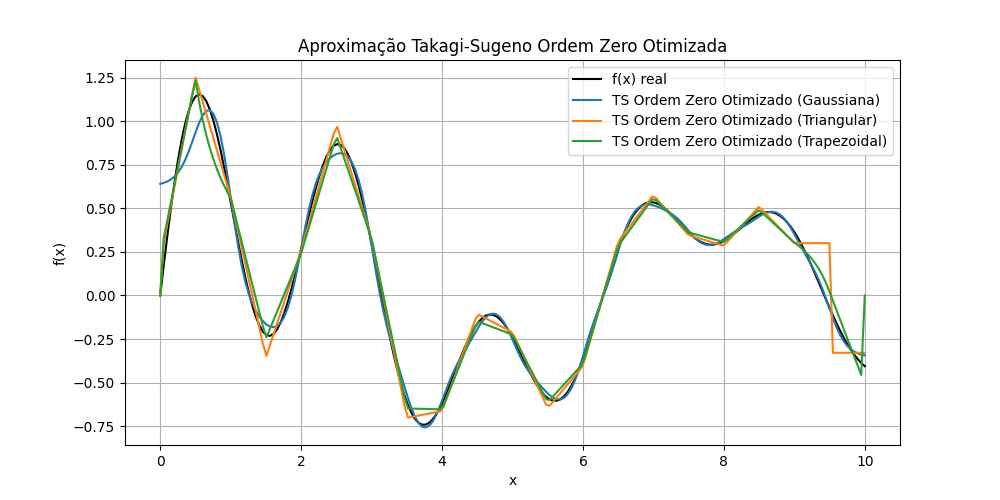
\includegraphics[width=0.45\textwidth]{../img/fx_aprox_ordem_zero_otimizada_takagi_sugeno2.png}
    \caption{Aproximação Takagi-Sugeno ordem zero após otimização dos consequentes para diferentes funções de pertinência.}
    \label{fig:ts_ordem_zero_otimizada}
\end{figure}

As Figuras~\ref{fig:ts_ordem_zero_otimizada_gaussiana}, \ref{fig:ts_ordem_zero_otimizada_triangular} e \ref{fig:ts_ordem_zero_otimizada_trapezoidal} detalham o resultado para cada função de pertinência:

\begin{figure}[!ht]
    \centering
    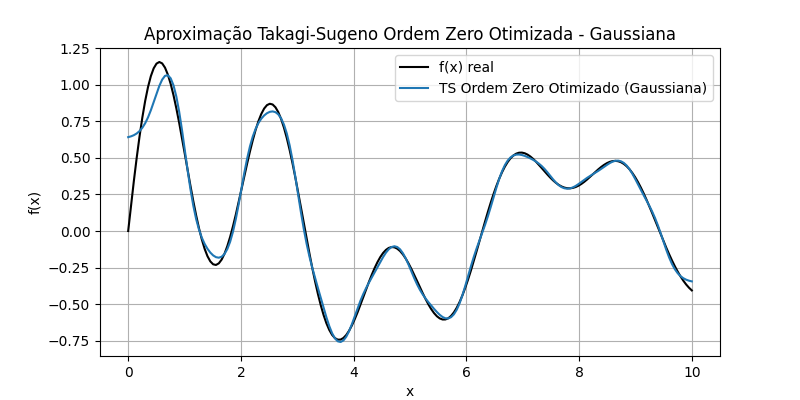
\includegraphics[width=0.45\textwidth]{../img/fx_aprox_ordem_zero_otimizada_gaussiana_takagi_sugeno2.png}
    \caption{Aproximação TS ordem zero otimizada - Gaussiana.}
    \label{fig:ts_ordem_zero_otimizada_gaussiana}
\end{figure}

\begin{figure}[!ht]
    \centering
    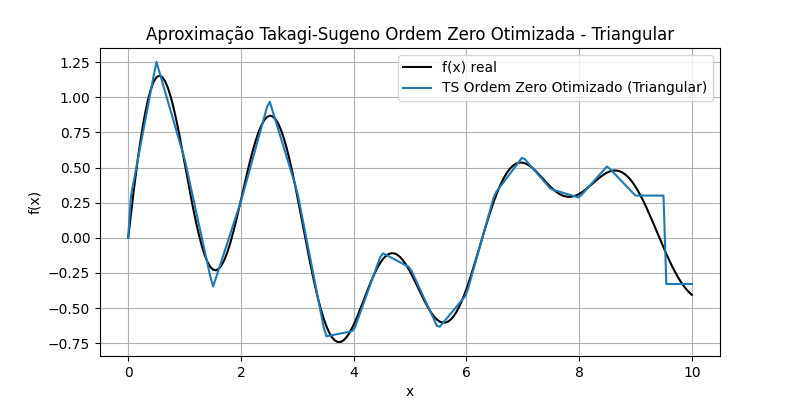
\includegraphics[width=0.45\textwidth]{../img/fx_aprox_ordem_zero_otimizada_triangular_takagi_sugeno2.png}
    \caption{Aproximação TS ordem zero otimizada - Triangular.}
    \label{fig:ts_ordem_zero_otimizada_triangular}
\end{figure}

\begin{figure}[!ht]
    \centering
    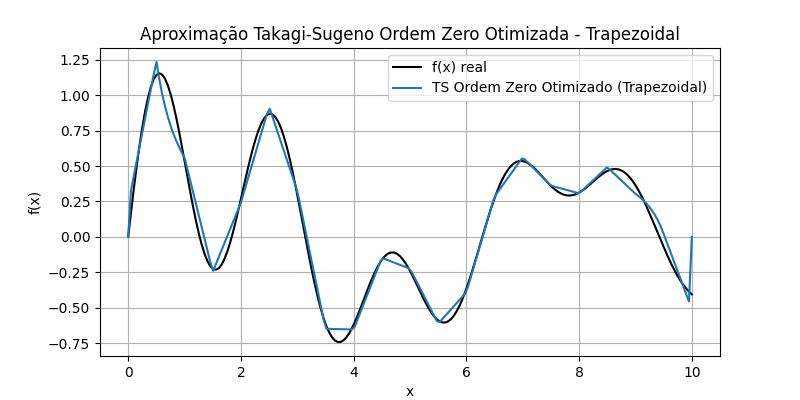
\includegraphics[width=0.45\textwidth]{../img/fx_aprox_ordem_zero_otimizada_trapezoidal_takagi_sugeno2.png}
    \caption{Aproximação TS ordem zero otimizada - Trapezoidal.}
    \label{fig:ts_ordem_zero_otimizada_trapezoidal}
\end{figure}

Observa-se que a otimização dos consequentes reduz significativamente o erro, tornando o modelo de ordem zero competitivo com o de primeira ordem, especialmente para funções de pertinência triangulares.